\chapter*{Cersion 2}
\label{chap:Technical CHallenges}
\renewcommand{\thesection}{\arabic{section}}
\setcounter{section}{0}

After my first attempts and some discussion with my supervisor i realized that the solution is to distribute the system and send the data wirelessly. This enables me to add additional sensors without having issues with the Wire library. However this increases the cost and complexity of each sensor slightly, since each sensor needs some sort of "brain", which handles the connection and communciation. 
However it reduces the complexity of the construction and the entire solution drasticly since it has single services talking ot each other and not an entier blob of logic. 

\section{Attempt 1}

The communication wase firstly achieved via WIFI since I know the protocol and can get it running swiftly. Also the esp32 I have been using has WIFI natively enabled. 
An issue with wireless communication is the synchronisation of the data flow. To simplify the process and due to lack of knowhow and time to achieve a correct synchronisation I will ignore it, while knowing the data might be timeshifted. 
This might be an issue when visualising and analysing the data, but will be tackled then.

Forthermore for the communication via WIFI a simple "Client Server" protocoll was used which has already been widely implement in ESP32.

Server Client Request: 
\begin{lstlisting}
String clientRequest(String input)
{
  Serial.println(input);
  String response = "\0";
  for (int i = 0; i < NUM_CLIENTS; i++)
  {
    WiFiClient client = server.available();
    client.setTimeout(50);
    if (client) {
      if (client.connected()) {
        client.println(input);
        data = client.readStringUntil('\r');  // received the server's answer
        Serial.println(data);
        if (data != "\0")
        {
          int Index = data.indexOf(':');
        
          CLIENT = data.substring(0, Index);
          ACTION = data.substring(Index + 1);
          Serial.println(data);
   
          if (CLIENT == "ACK")
          {
            response = ACTION;
          }

          //client.flush();
          //data = "\0";
        }
      }else{
        Serial.println("client not connected");
      }
    }
    else{
        Serial.println("client null or false");
      }
  }
\end{lstlisting}

Client Loop:

\begin{lstlisting}
void loop () {
  if (!client.connect(server, 80)) {
    while (WiFi.status() != WL_CONNECTED) {
      Serial.print(".");
      delay(500);
    }
    Serial.print("+");
    delay(100);
    return;
  }
  data = client.readStringUntil('\r');  // received the server's answer
  Serial.println(data);
  if (data != "\0")
  {
    int Index = data.indexOf(':');

    CLIENT = data.substring(0, Index);
    ACTION = data.substring(Index + 1);

    if (CLIENT == CLIENT_NAME)
    {
         client.println("ACK:" + getData());
      
    }else{
        client.println("\0");
    }

    client.flush();
    data = "\0";
  }
}
\end{lstlisting}

The Data will be sent 10 times per second for evaluation purposes. 
However I hope and think this can be reduced, since we hopefully will not need that much data to determine how to usere i positioned. This would enable us to aggregate the data on the devices, which is a benefit only achievable by the current configuration of "Smart-sensors".

The Data is saved onto an SD Card, this works well and enables to analyse de Data afert measuring it for a while. This Concept worked quite well, hovewer it has some major flaws. 

\section{Flaws of Attempt A}

The Idea of saving all the data locally came with the plan to have everything locally which then in a further step could be sent the a smartphone or a laptop without any interent. Maybe with bluetooth or a local hotspot. 

During the development and testing of this concept, it turned out that the client server network was not very stable and it required much more hardware than i woud have liked. 
The Server needed a few modules for it to work.

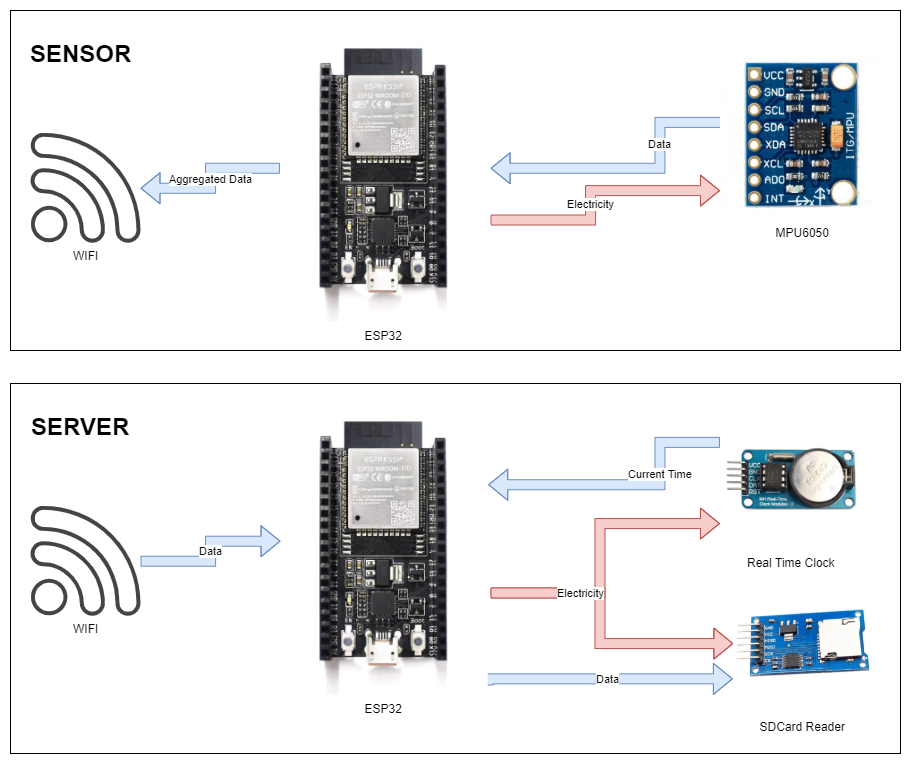
\includegraphics[width=\linewidth]{images/CommunicationDiagrammExplenation.png}

This does not sound like mucht but both of these elementes are quite complex and need to be configured additionally. This felt like quite the hassle and i sonn realized i need to find a new way to communicate.

Beside these technical issues the data transfer during the development phase, where bluetooth or hotspot was avaialble was quite awkward since the device need to be stopped and the data needed to be analysed in a spereate step. 


\begin{center}
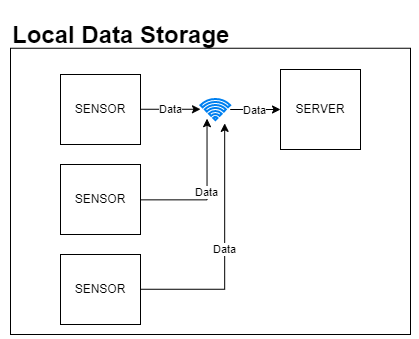
\includegraphics[width=0.5\textwidth]{images/CommunicationDiagrammLocal.png}
 \end{center}
After working with it for a while I tried to find a much simpler way, which is closer to the goal of a simple and affordable sensor set. To Tackle the issues with the client server network i first thought of using a simple http request, which would have a bit more overhead but would be more stable. This however didn't feel right and I realized that the solution, was something I already was quite familiar with. A simple MQTT Broker. 



\section{Atempt B}

After this first attempt i knew how to handle the message and date from the sensors which helped greatly. 
The Communication in my new attempt was handled with a simple MQTT Broker, which can be setup for free within seconds. For my endeavours I used cloudmqtt.com which is completly free and easy to apply. 


\begin{center}
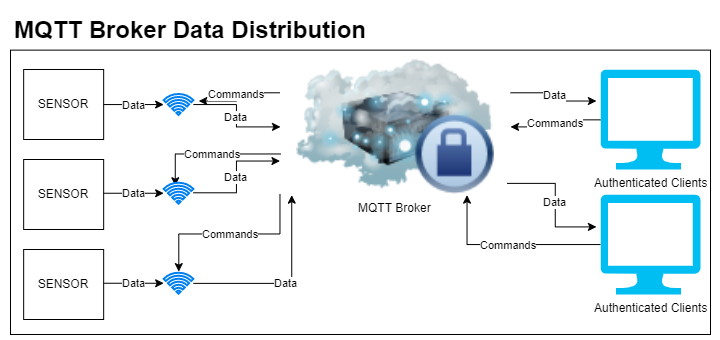
\includegraphics[width=0.8\textwidth]{images/CommunicationDiagrammMQTT.png}
\end{center}
MQTT uses a simple publish subscribe protocoll which I have already implemented a few times.
Below you see the whole setup and loop code, which is almost readable thanks to helper functions:
\begin{lstlisting}
void setup() {
  Serial.begin(115200);
  Wire.begin();
  USERID = getRegisterdUserid();
  setupMPU();
  setupWifi();
  client.setServer(mqtt_server, mqtt_port);
  client.setCallback(callback);

  strcpy(fullsubtopic, TOPIC); 
  strcat(fullsubtopic, USERID);
  strcat(fullsubtopic, SUB);
  
  strcpy(fullpubtopic, TOPIC); 
  strcat(fullpubtopic, USERID);
  //strcat(fullpubtopic, PUB);
  
  while (!client.connected()) {
   reconnect();
  }
  startMillis = millis(); 
  getData();
}

void loop () {
  client.loop();
  currentMillis = millis();  //get the current "time" (actually the number of milliseconds since the program started)
  if (currentMillis - startMillis >= period)  //test whether the period has elapsed
  {
    Serial.println("trying to send");
    char * message = getMessage();
    publish(message);
    Serial.println(message);
    startMillis = currentMillis;  //IMPORTANT to save the start time of the current LED state.
  }
 getData();
 }
\end{lstlisting}

This loop collected the data into an average in "getData()" function
\begin{lstlisting}
void getData(){
  if(readByte(MPU6050_ADDRESS, INT_STATUS) & 0x01) {  // check if data ready interrupt
    readAccelData(accelCount);  // Read the x/y/z adc values
    getAres();
    ax = (float)accelCount[0]*aRes - accelBias[0];  // get actual g value, this depends on scale being set
    ay = (float)accelCount[1]*aRes - accelBias[1];   
    az = (float)accelCount[2]*aRes - accelBias[2];  
    readGyroData(gyroCount);  // Read the x/y/z adc values
    getGres();
    gx = (float)gyroCount[0]*gRes - gyroBias[0];  // get actual gyro value, this depends on scale being set
    gy = (float)gyroCount[1]*gRes - gyroBias[1];  
    gz = (float)gyroCount[2]*gRes - gyroBias[2];  
    tempCount = readTempData();  // Read the x/y/z adc values
    temperature = ((float) tempCount) / 340. + 36.53; // Temperature in degrees Centigrade
 
    accelVal[0] = ax;
    accelVal[1] = ay;
    accelVal[2] = az;
    gyroVal[0] = gx;
    gyroVal[1] = gy;
    gyroVal[2] = gz;
    setAvg();
    
   }
}
void setAvg(){
    for (int i = 0; i < 3; i++){
      avgAccelVal[i] = (avgAccelVal[i] + accelVal[i])/2;
      avgGyroVal[i] = (avgGyroVal[i] + gyroVal[i])/2;
  }
}
\end{lstlisting}
 and created a json from the collected data in the "getMessage()" function which was sent every second: 
\begin{lstlisting}
char* getMessage(){
  char* a = "{ \"id\": \"";
  char* b = "\", \"acc\":[";
  char* c= "], \"gyro\":[";
  char* d= "]}"; 
  char accelbuff[64];
  char gyrobuff[64];
  Serial.println("loading data to buffers");
  char* loc = accelbuff;
   size_t tempLen;
   int i = 0;
   for(i = 0; i < DIM(avgAccelVal)-1; ++i)
    {
        snprintf(loc, 12, "%f,", avgAccelVal[i]);
        tempLen = strlen(loc);
        loc += tempLen;
    }
   snprintf(loc, 12, "%f", avgAccelVal[i+1]);
   tempLen = strlen(loc);
   loc += tempLen;
   loc = gyrobuff;
   for(i = 0; i < DIM(avgGyroVal)-1; ++i)
    {
        snprintf(loc, 12, "%f,", avgGyroVal[i]);
        tempLen = strlen(loc);
        loc += tempLen;
    }
  snprintf(loc, 12, "%f", avgGyroVal[i+1]);
  tempLen = strlen(loc);
  loc += tempLen;
  strcpy(messagebuffer, a ); 
  strcat(messagebuffer, DEVICEID);
  strcat(messagebuffer, b);
  strcat(messagebuffer, accelbuff);
  strcat(messagebuffer, c);
  strcat(messagebuffer, gyrobuff);
  strcat(messagebuffer, d);
  return messagebuffer;
}
\end{lstlisting}
As you can see the creation of the message, was almost the most complex part of the implementation. This was due to the fact, that the mqtt Library could not handle "arduino" Strings and therefored need char* which are a mess to work with. Nontheless after some tinkering i finally managed to get a nice JSON message over the MQTT Broker: 
\begin{lstlisting}
{ 
    "id": "SENSOR-XSZ", 
    "acc":[-0.003835,0.001486,0.056012],
    "gyro":[0.056012,0.240598,0.038814]
}
\end{lstlisting}

Additionally I enabled all devices to be calibrated remotely. This since when i put these devices on I will ned to calibrate them after they are set in position. This is quite a simple task with MQTT since the clients can simply subscribe to a topic, from which they get messages: 

\begin{lstlisting}
void callback(char* topic, byte* message, unsigned int length) {
  Serial.print("Message arrived on topic: ");
  Serial.print(topic);
  Serial.print(". Message: ");
  String command;
  
  for (int i = 0; i < length; i++) {
    Serial.print((char)message[i]);
    command += (char)message[i];
  }
  if(command == "calibrate"){
    calibrateMPU6050(gyroBias, accelBias); // Calibrate gyro and accelerometers, load biases in bias registers  
    initMPU6050(); 
    Serial.println("MPU6050 initialized for active data mode....");
  }
}
\end{lstlisting}
This callback gets registered when connecting to the mqtt broker.



\subsection{Benefits Version B}

The Benefint of managing the messages via a MQTT Broker was that I could get the messages and work with them from any device with an Internet connection. This means that any calculation heavy tasks can be done from a "real" computer which handles these much better. 

This also enabled me to visualize and analyze the data in realtime which made it much easier. 

Furthermore it also achieves the goal of being cheap and affordable. Since we now only need MPU6050 and microntrollers to send the data and this can be setup much easier than with an ESP32 "server".

This also means that there does not need to be any more logic on the devices itself since everyhting can be done from a Computer. Maybe some sort of vibration device will be added which however also can be activated via the MQTT Broker. 

The Fact that these sensors now can simply send data without knowing where they are or what exactly they are measuring might open quite a lot of doors. I will get further into that in a later chapter.

\subsection{Backdraws Version B}

The Obvious backdraw is, that the sensors need to have a constant interent connection. This is obviously not great, especially when we try to develop something for an every usage since we are somewhat bound to a single place. 

Furthermore if used as a product, these sensors would need to be registered first bevor usage, this does increase complexity for a first usage however simplifes setup greatly.


\section{Identifying Posture}

The biggest hurdle, was and still is identifying and correctly analysing the data. I have had several different approaches on how to interpret and visualise the data. During my first attempt (Attempt A) i tried to visualised the data in two ways, with Python and Power BI.

Firstly I transformed the data into a \acrshort{csv} (\gls{CSV}). CSV is a commonly used format viable for many different applications

According to the datasheet of the MPU6050 the collected data is "g-force". The accelerometer measure in mg and the gyroscope in \degree/s. 

\begin{figure}[h]
\begin{center}
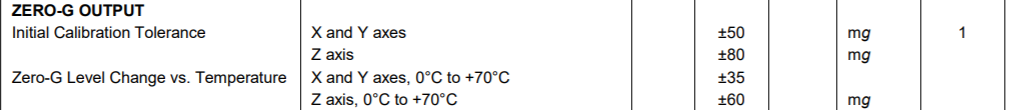
\includegraphics[width=\linewidth]{images/MPU6050_DATA.png}
  \end{center}
  \caption{MPU Datasheet}
  \label{fig:MPUDatasheet}
\end{figure}

The entire documentation can be found online \cite{MPU6000D59:online}.

\subsection{Visualising with Python}

I tried to visualise the data using \gls{Python} since it was recommended on a few forums and seamed to be feasible for this task. It actually did work quite well and I have achieved within 2 Days with Python. I have never worked with python before and was happy that I managed to use and apply it within days. 

\begin{figure}[h!]
\begin{center}
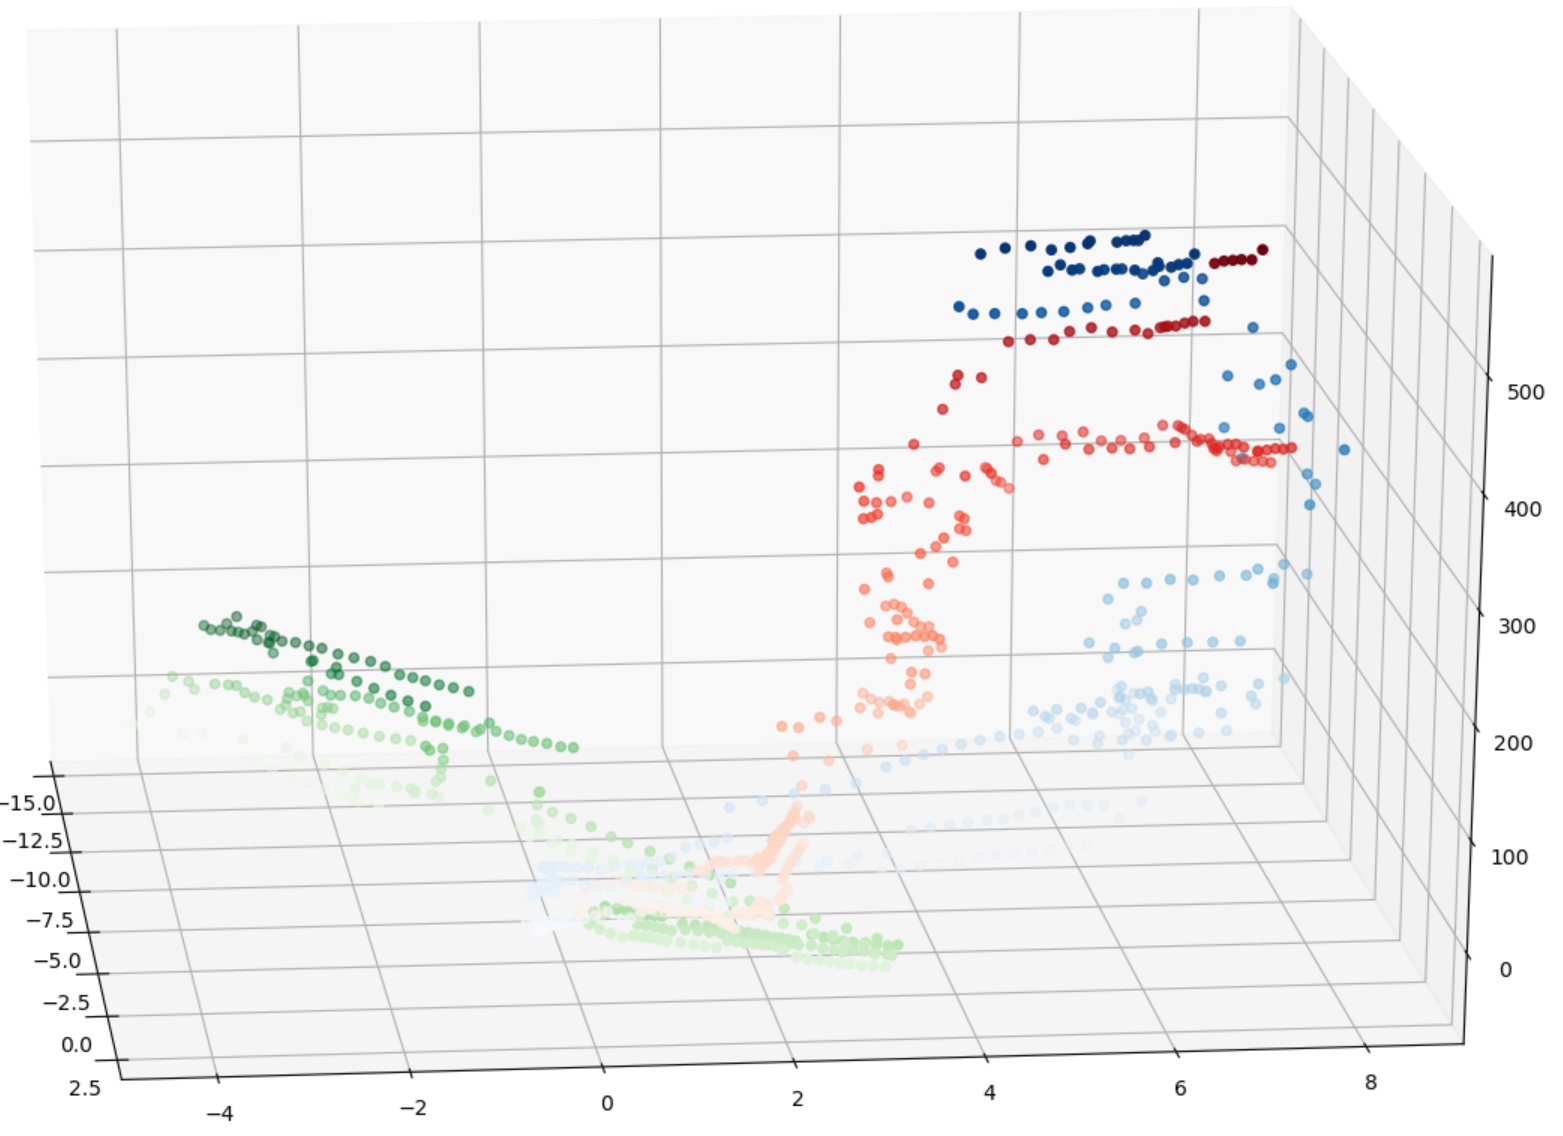
\includegraphics[width=0.6\linewidth]{images/PyVisualisation.png}
  \end{center}
  \caption{Python Visualisation}
  \label{fig:PythonVisualisation}
\end{figure}

Visualised you see my first attempt in figure \ref{fig:PythonVisualisation}, showing movement of 3 sensors with the data of the accelerometers. The sensors were attached to my shirt with scotch. This is not a perfect solution, which is visible in the different orientation of the green dots. 

Here I tried to add up the movement from the accelerometers to see how this stacks up. The Data was not very helpful and i tried to anime the accelerometer data directly to see how it changes, this was a bit clearer but still very hard to interpret since it was static data. 

To visualise I used numpy and matplotlib which are quite handy but still took some time the get used to.
The data was simple display on a grapth (ax) from np arrays:

\begin{lstlisting}
ax.scatter3D(XSXAcc[:,0],XSXAcc[:,1],XSXAcc[:,2], c=XSXAcc[:,2], cmap='Reds')
ax.scatter3D(XSYAcc[:,0],XSYAcc[:,1],XSYAcc[:,2], c=XSYAcc[:,2], cmap='Blues')
ax.scatter3D(XSZAcc[:,0],XSZAcc[:,1],XSZAcc[:,2], c=XSZAcc[:,2], cmap='Greens')
\end{lstlisting}

\subsection{Visualising with Power BI}

\gls{Power BI} is a very powerful tool which I was already used to, since we used it at work to visualise project data and quality gates. Therefore it was much easier for me to visualise the data.

During different attempts of visualising the data i realised, it made sense to visualise it with a 2d graph, since the three dimensional visualisation did not offer any real benefits. Furthermore during this visualisation I also quickly saw, that the data collected had to be incorrect, since the accelerometer should never fluctuate as much as it did. The error was in my code and was quickly fixed, however I still had issues making conclusions from this static data.

\begin{figure}[h]
\begin{center}
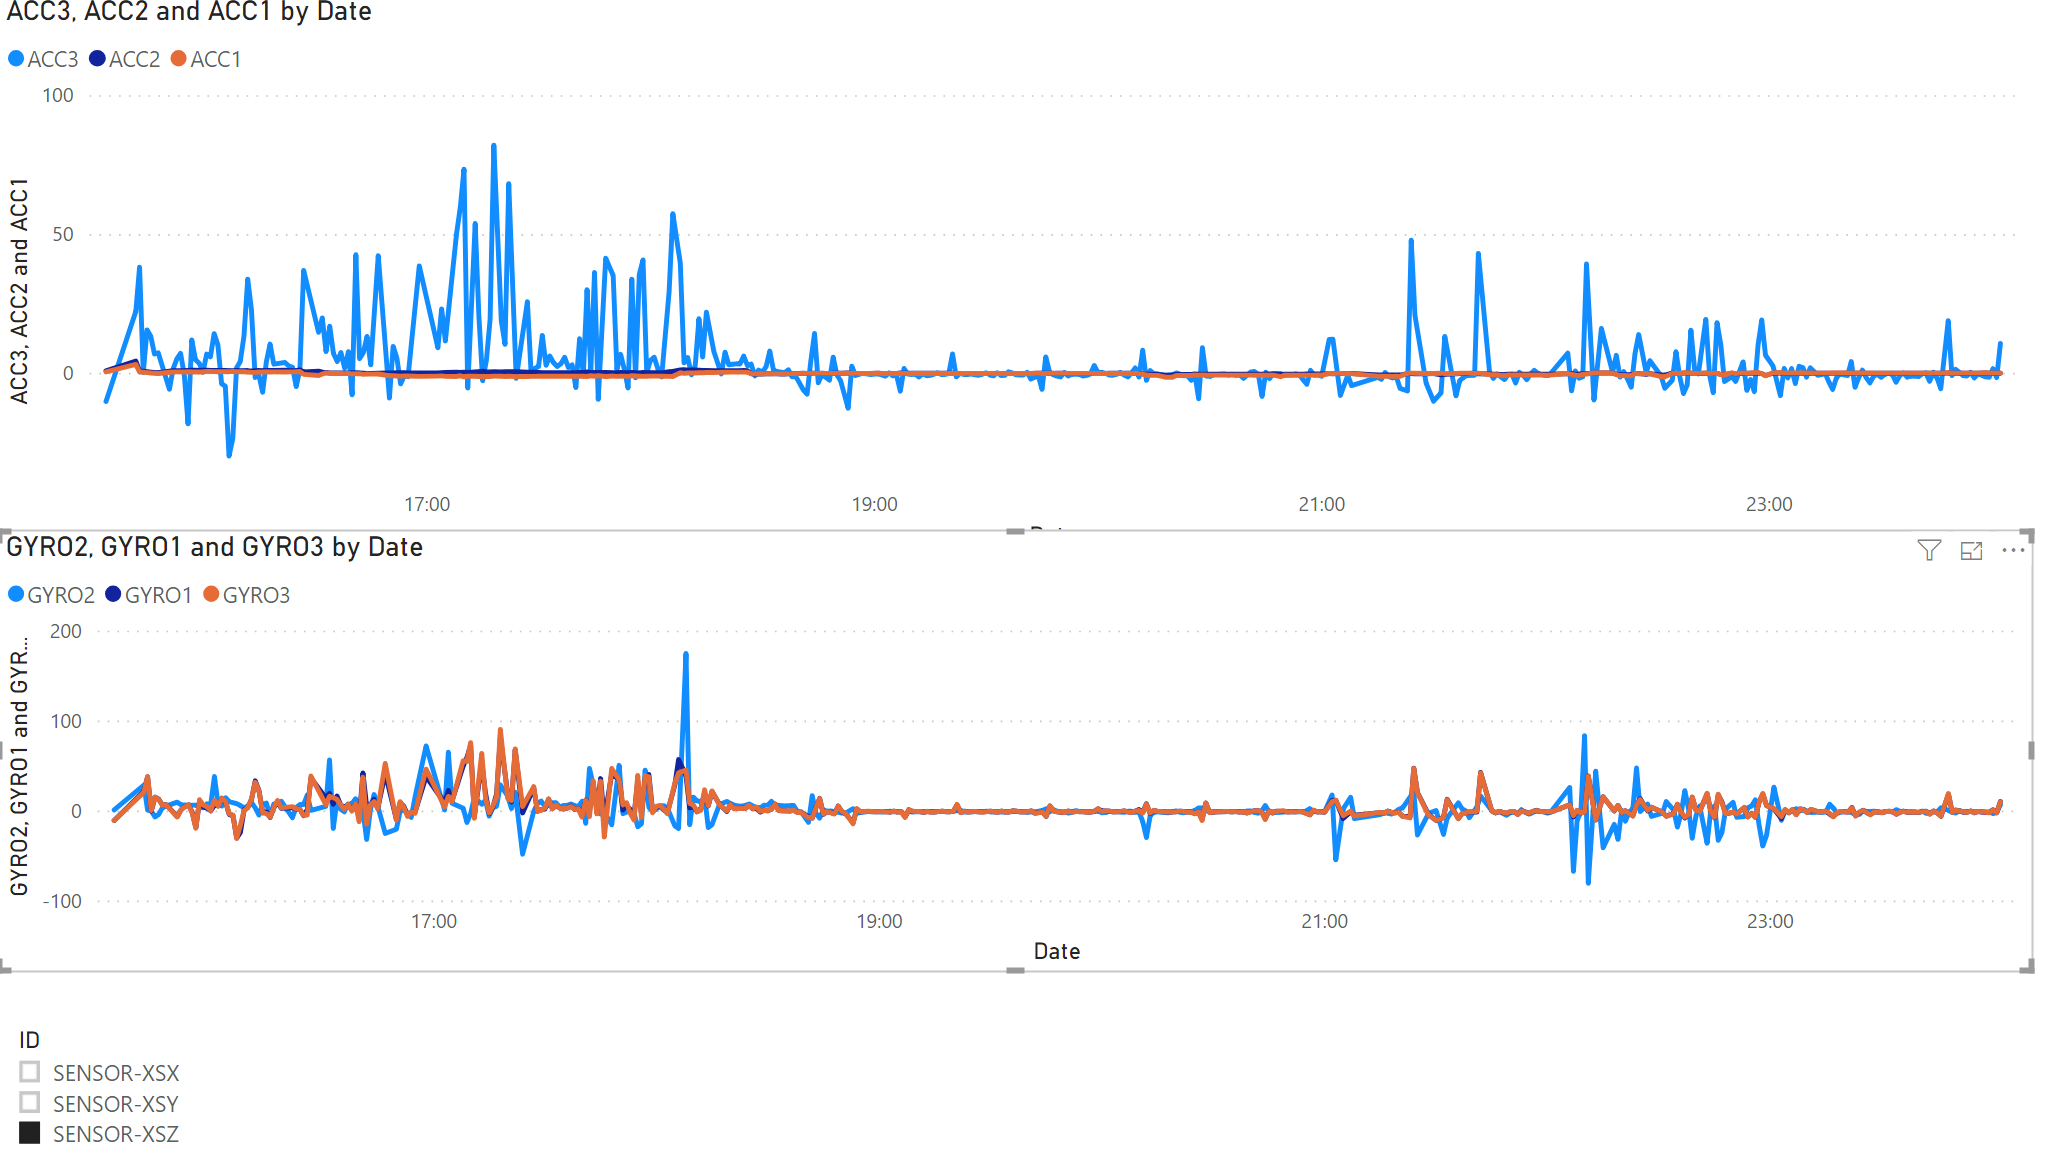
\includegraphics[width=0.7\linewidth]{images/PowerBIVisualisiation.png}
  \end{center}
  \caption{Power BI Visualisation}
  \label{fig:PowerBIVisualisation}
\end{figure}

\newpage


